\section{Results and interpretation}
\label{sect:stat}
The observed data and predicted background yields for the four signal regions are summarized in Table~\ref{tbl:yieldSysSummary}. 
\begin{table}[!htb]
\begin{center}
%\begin{tiny}
\caption{Data yields and background predictions with uncertainties in the four signal regions of the search. 
%The first two lines are based on Monte Carlo simulation, when for the first row, a validation against data is also done. 
%The last two rows are data driven, but the ``Fake'' for the \tauTau channel is not completely data driven.
%The uncertainties are systematic, unless when there are two parts, the first part is statistics.
The uncertainties are reported in two parts, the statistical and systematic uncertainties, respectively. 
%For \wjets in \tauTau channel, the full uncertainty is
%reported and considered as systematic for ``SM Total''.
The \wjets and QCD multijet main backgrounds are derived from data as described in Section~\ref{sect:bkg}; 
the abbreviation ``VV'' refers to diboson events. The yields for three signal points representing the low, medium, and high $\Delta m$
are also shown. SUSY(X, Y) stands for a SUSY signal with ${\rm{m}}_{\chione}$ = X\GeV and ${\rm{m}}_{\neutralino}$ = Y\GeV.}
\begin{tabular}{|c|c|c|c|c|}
\hline
	           & \eTau & \muTau & \tauTau \binone & \tauTau \bintwo \\
\hline
  DY               & 0.19 $\pm$ 0.04 $\pm$ 0.03 & 0.25 $\pm$ 0.06  $\pm$ 0.04  &  0.56 $\pm$ 0.07 $\pm$ 0.12 & 0.81 $\pm$ 0.56 $\pm$ 0.18  \\
tX, VV, hX  & 0.03 $\pm$ 0.03 $\pm$ 0.02 & 0.19 $\pm$ 0.09  $\pm$ 0.09  &  0.19 $\pm$ 0.03 $\pm$ 0.09 & 0.75 $\pm$ 0.35 $\pm$ 0.38  \\
\wjets             & 3.30$_{- 3.30}^{+ 3.35}$ $\pm$ 0.56 & 8.15 $\pm$ 4.59  $\pm$ 1.53  &  0.70 $\pm$ 0.21 $\pm$ 0.55 & 4.36 $\pm$ 1.05 $\pm$ 1.63  \\
QCD multijet       &             -              &            -                 &  0.13 $\pm$ 0.06 $\pm$ 0.21 & 1.15 $\pm$ 0.39 $\pm$ 0.74  \\
\hline
SM total           & 3.52 $\pm$ 3.35 $\pm$ 0.56 & 8.59 $\pm$ 4.59  $\pm$ 1.53  &  1.58 $\pm$ 0.23 $\pm$ 0.61 & 7.07 $\pm$ 1.30 $\pm$ 1.84  \\
\hline
Observed           &               3            &                5             &             1               & 2     \\\hline  
SUSY(380, 1)        & 2.14 $\pm$ 0.08 $\pm$ 0.38 & 2.16 $\pm$ 0.08  $\pm$ 0.39  &  4.10 $\pm$ 0.10 $\pm$ 0.90 & 1.10 $\pm$ 0.05 $\pm$ 0.27 \\
SUSY(240, 40)       & 1.43 $\pm$ 0.19 $\pm$ 0.21 & 0.96 $\pm$ 0.14  $\pm$ 0.14  &  4.35 $\pm$ 0.27 $\pm$ 0.91 & 3.60 $\pm$ 0.25 $\pm$ 0.83 \\
SUSY(180, 60)       & 0.12 $\pm$ 0.04 $\pm$ 0.02 & 0.04 $\pm$ 0.02  $\pm$ 0.01  &  0.73 $\pm$ 0.11 $\pm$ 0.17 & 2.36 $\pm$ 0.17 $\pm$ 0.54 \\
\hline
\end{tabular}
\label{tbl:yieldSysSummary}
\end{center}
\end{table}

There is no evidence for an excess of events with respect to the predicted SM values in any of the signal regions. In \bintwo, two events are observed while 7.07 events are expected. The dominant background source is \wjets events. As a cross-check, data and the prediction in the sideband (200 $< \SumMT <$ 250\GeV) are studied: 13 events are observed with an expectation of 17.1 $\pm$ 5.0 (stat+syst) events. 
This result indicates that the difference between the observed and predicted event yields in \bintwo can be attributed to a downward fluctuation in the data.

Figure \ref{fig:yield_final}
\begin{figure}[!htb]
\centering
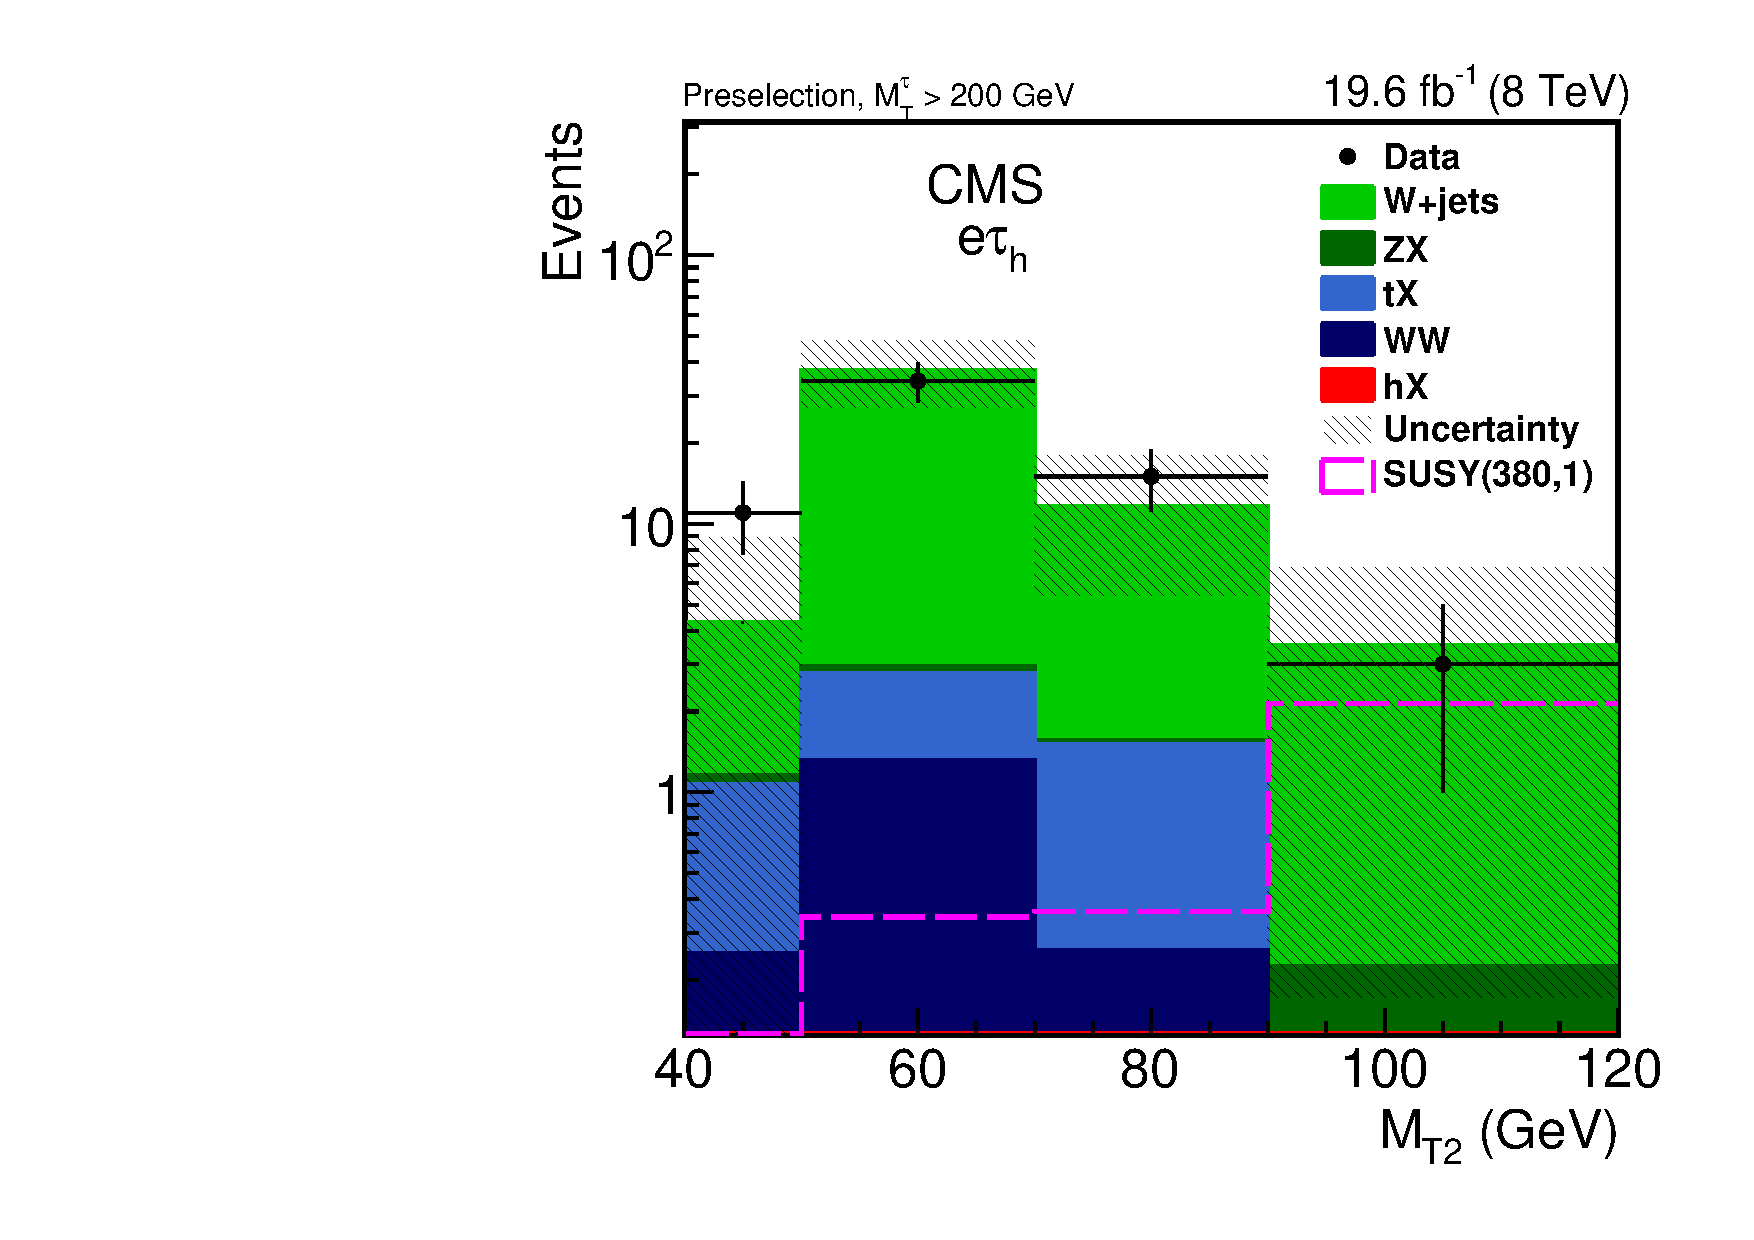
\includegraphics[width=0.475\textwidth,keepaspectratio=true]{StatisticsFig/MT2_tauMTgt200_DDFakeEleTau.pdf}
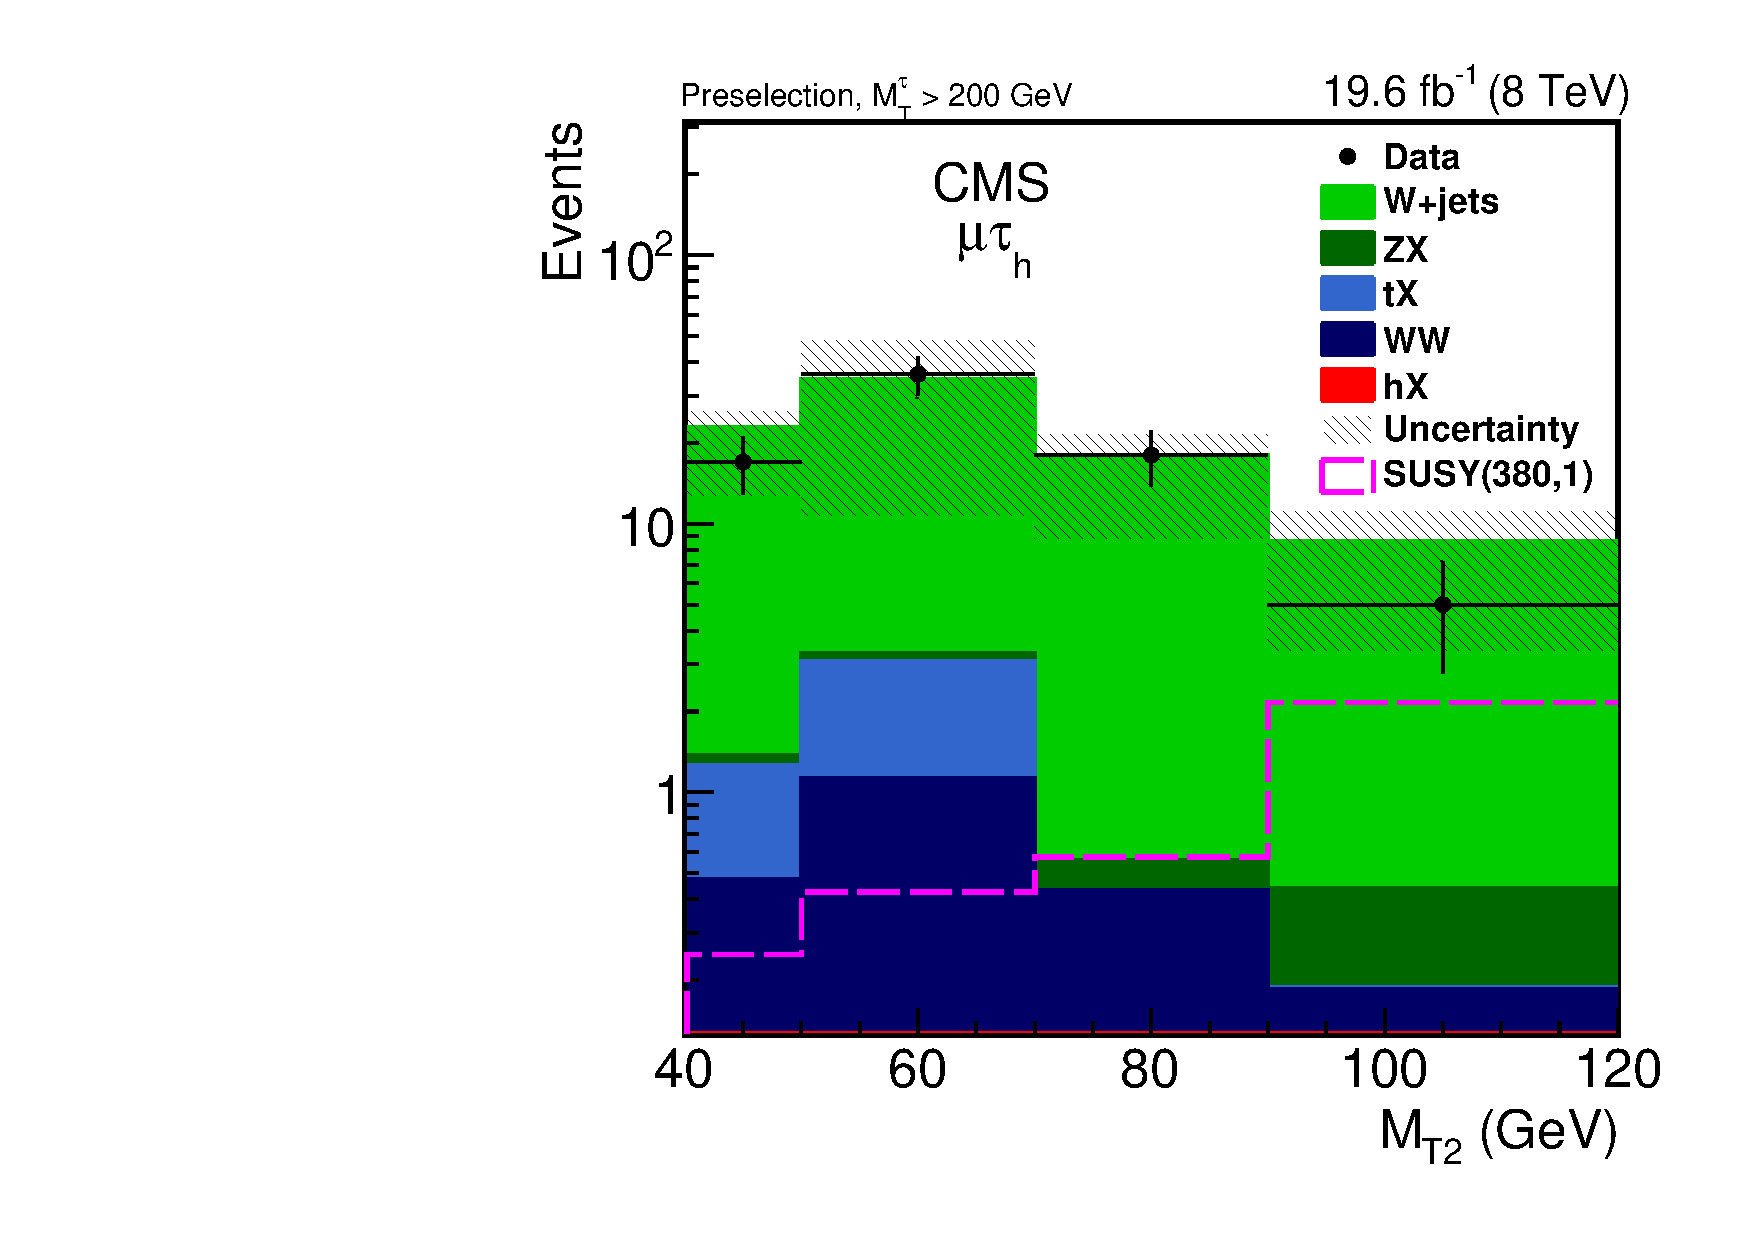
\includegraphics[width=0.475\textwidth,keepaspectratio=true]{StatisticsFig/MT2muTau_tauMTgt200_DDFake.pdf}
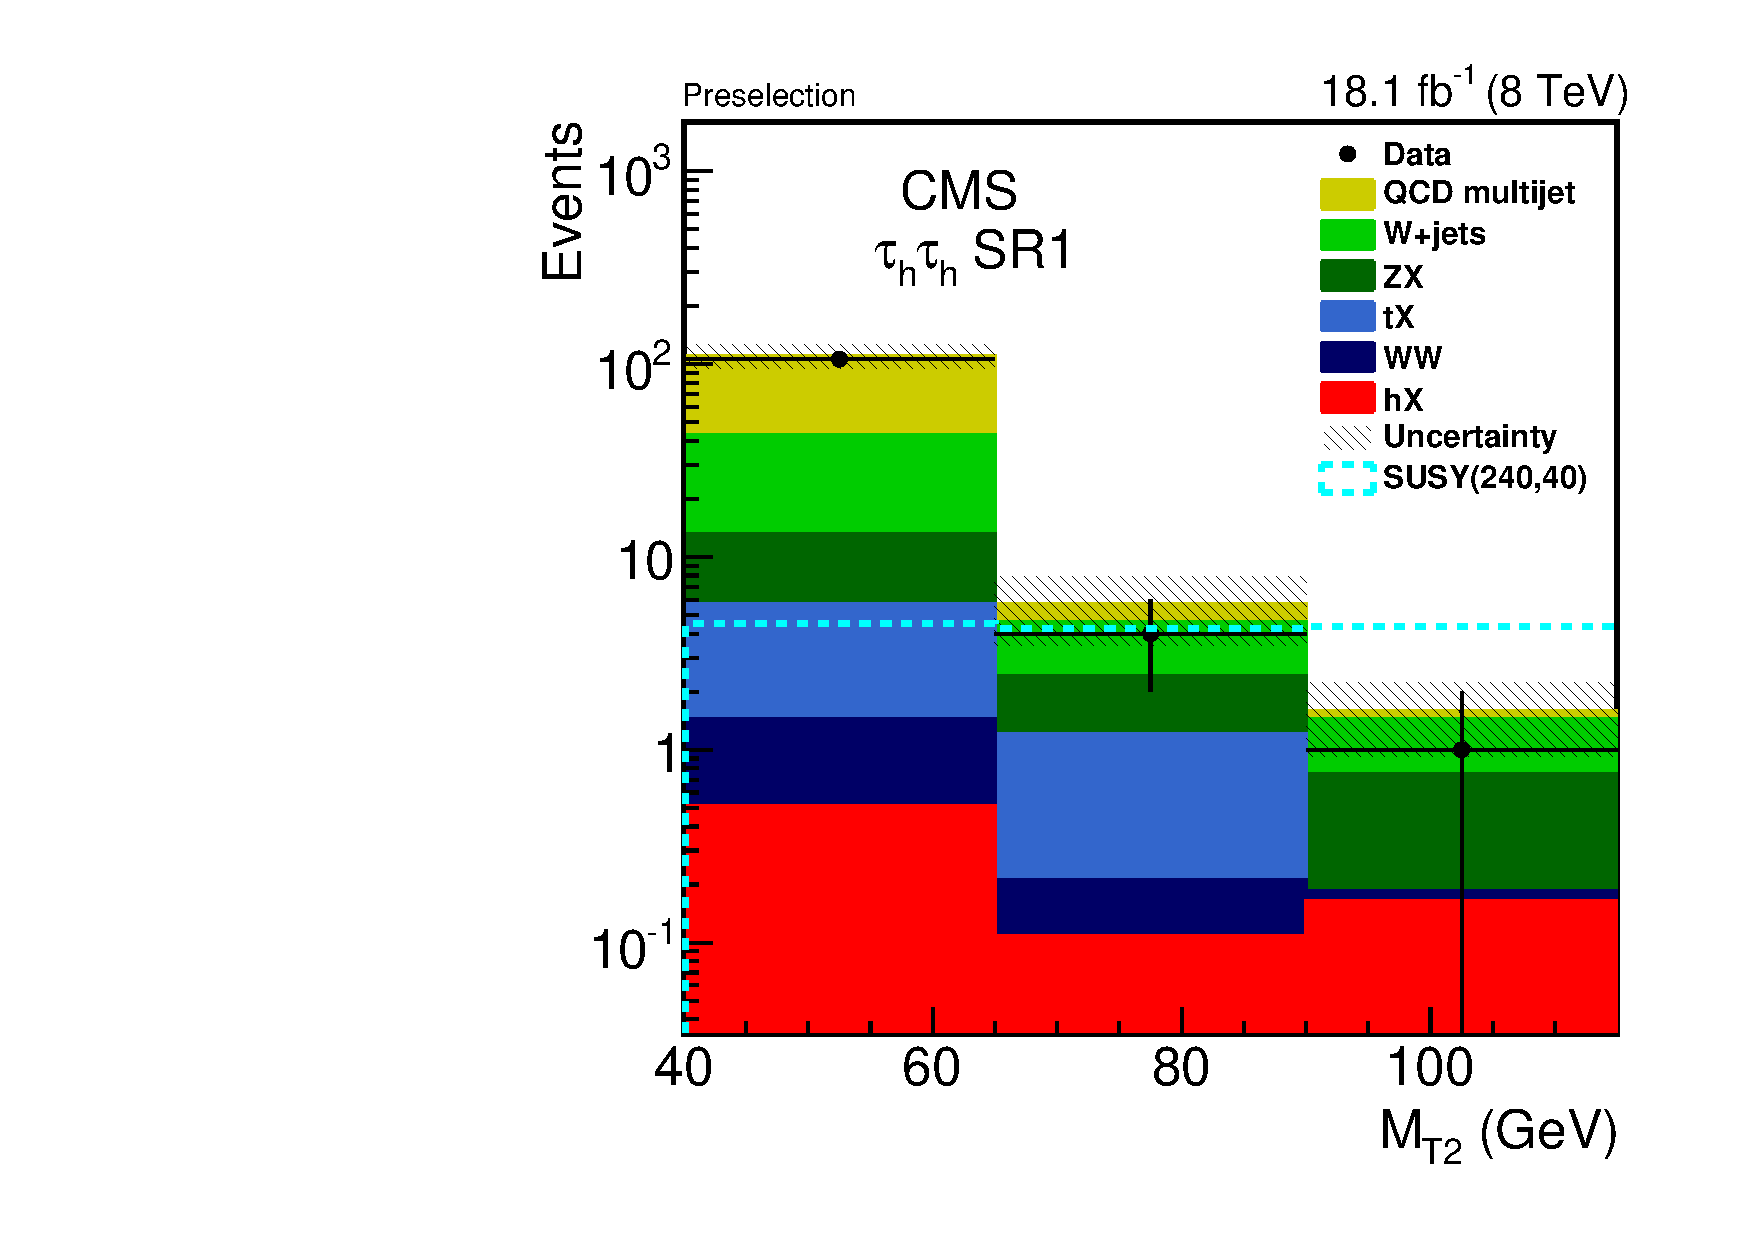
\includegraphics[width=0.475\textwidth,keepaspectratio=true]{StatisticsFig/QCDWestimation_bin1.pdf}
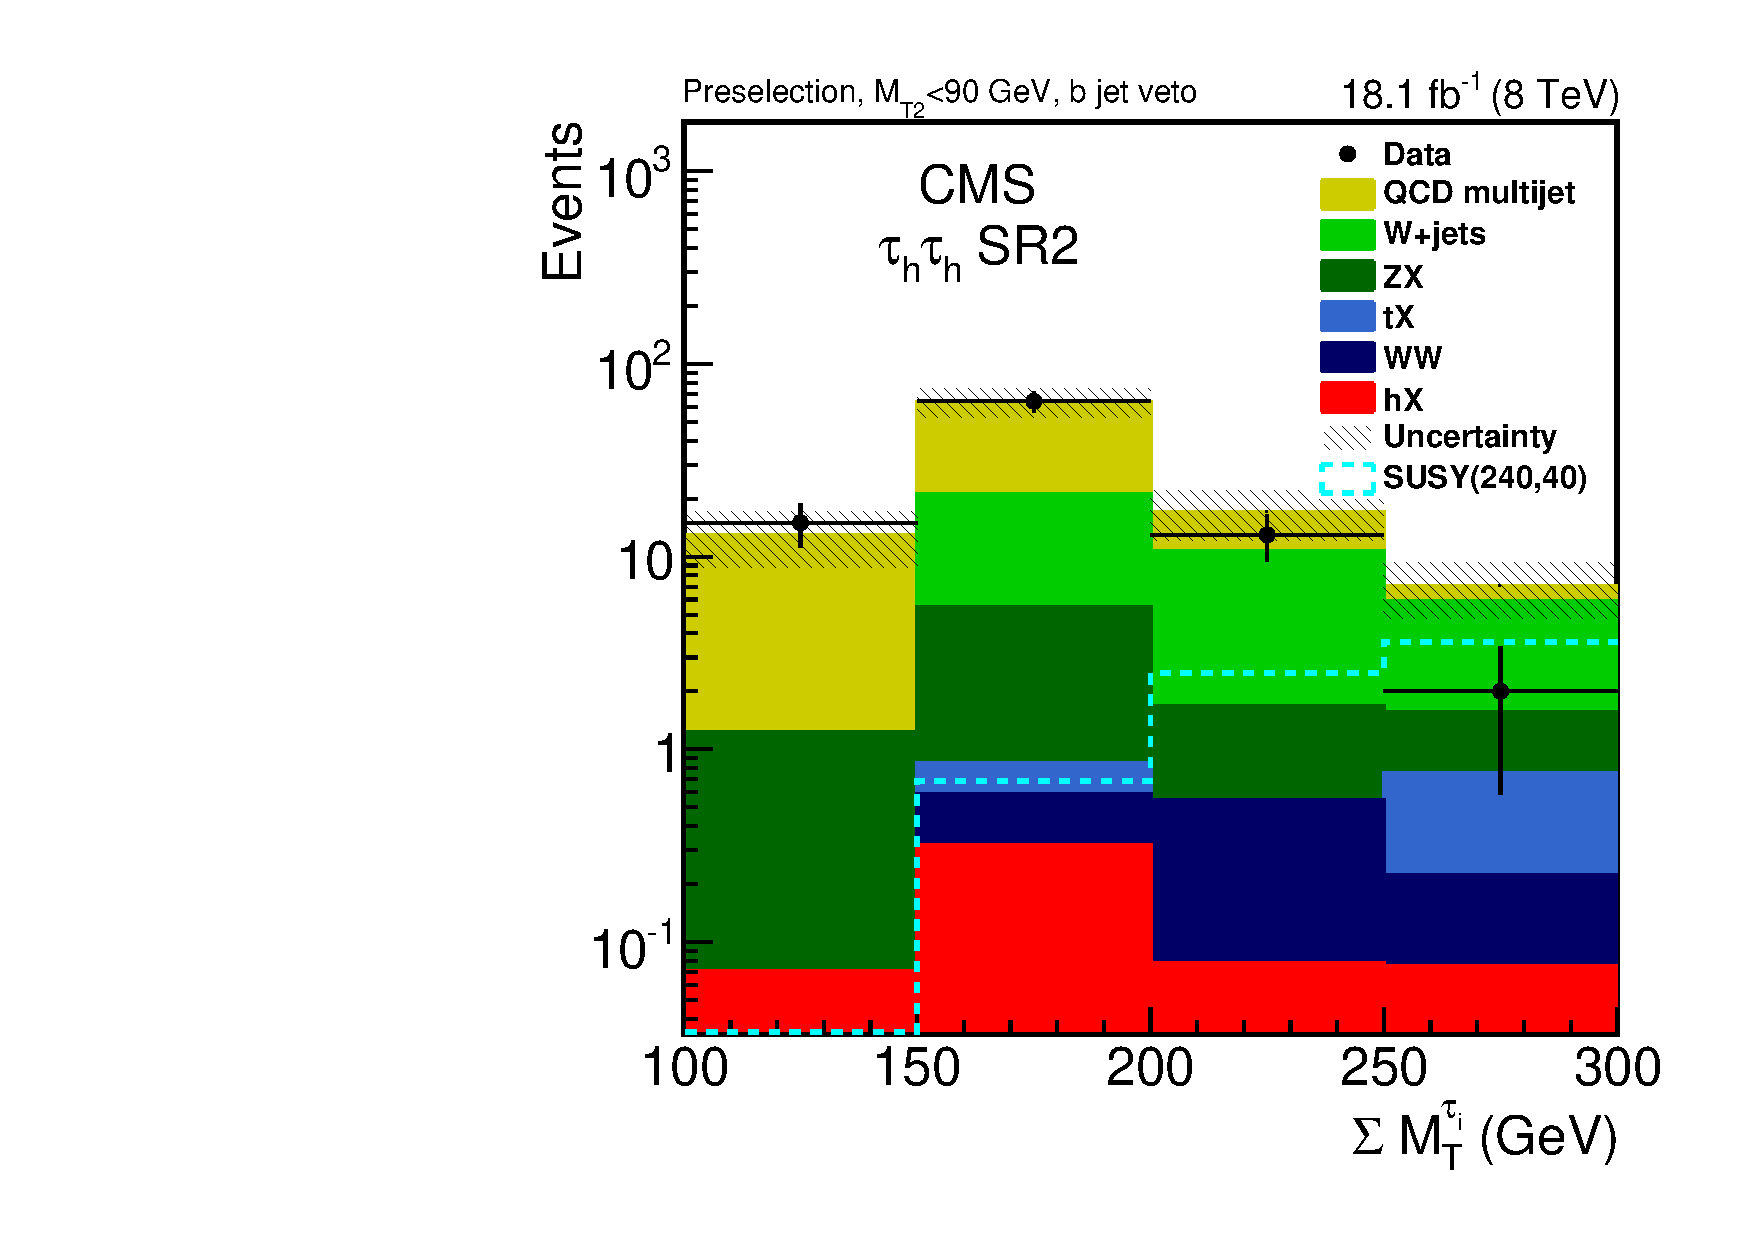
\includegraphics[width=0.475\textwidth,keepaspectratio=true]{StatisticsFig/QCDWestimation_bin2.pdf}
\caption{The data yield is compared with the SM expectation. In different signal regions, 
when a background estimate from data is available, it is used instead of simulation, as described in the text. The signal distribution for a high $\Delta m$ scenario with ${\rm{m}}_{\chione}$ = 380\GeV and ${\rm{m}}_{\neutralino}$ = 1\GeV is compared with the yields of \leptonTau channels while a scenario with lower $\Delta m$ (${\rm{m}}_{\chione}$ = 240\GeV and ${\rm{m}}_{\PSGczDo}$ = 40\GeV) is chosen for the comparison in \tauTau channels. The higher values of \mttwo or \SumMT are included in the last bins. The shown uncertainties include the quadratic sum of the statistical and systematic uncertainties.}
\label{fig:yield_final}
\end{figure}
compares the data and the SM expectation in four search regions. The top row 
shows the \mttwo distributions in the \leptonTau channels. 
In these plots, the QCD multijet, \wjets, and misidentified lepton contribution from other channels 
are based on the estimate described in Section \ref{sect:bkgFake} and labeled as \wjets.
%The QCD multijet contribution is very low for these channels and is included in the ``WX'' background estimate.
The bottom row shows the \mttwo and \SumMT distributions in the two different signal regions of the \tauTau channel. 
The QCD multijet contribution in these plots is obtained using control samples in data, as described in 
Section \ref{sect:bkgQCD}. The \wjets contribution in 
the last bin of the bottom plots is described in Section \ref{sect:bkgW}, while the contribution to other bins is based on simulated events.
The uncertainty band in these four plots includes both the statistical and systematic uncertainties.

There is no excess of events over the SM expectation.  These results are interpreted in the context
of a simplified model of chargino pair production and decay, which is described in Section~\ref{sect:MCSamples} and corresponds 
to the left diagram in Fig.~\ref{fig:Productions}. 

A modified frequentist approach, known as the LHC-style CL$_s$ criterion \cite{read:CLs,Junk:1999kv,ATLAS:2011tau}, is used to 
set limits on cross sections at a 95\% confidence level (CL).
The results on the excluded regions are shown in Fig.~\ref{fig:limit_final}. 
\begin{linenomath}
\begin{figure}[!htb]
\centering
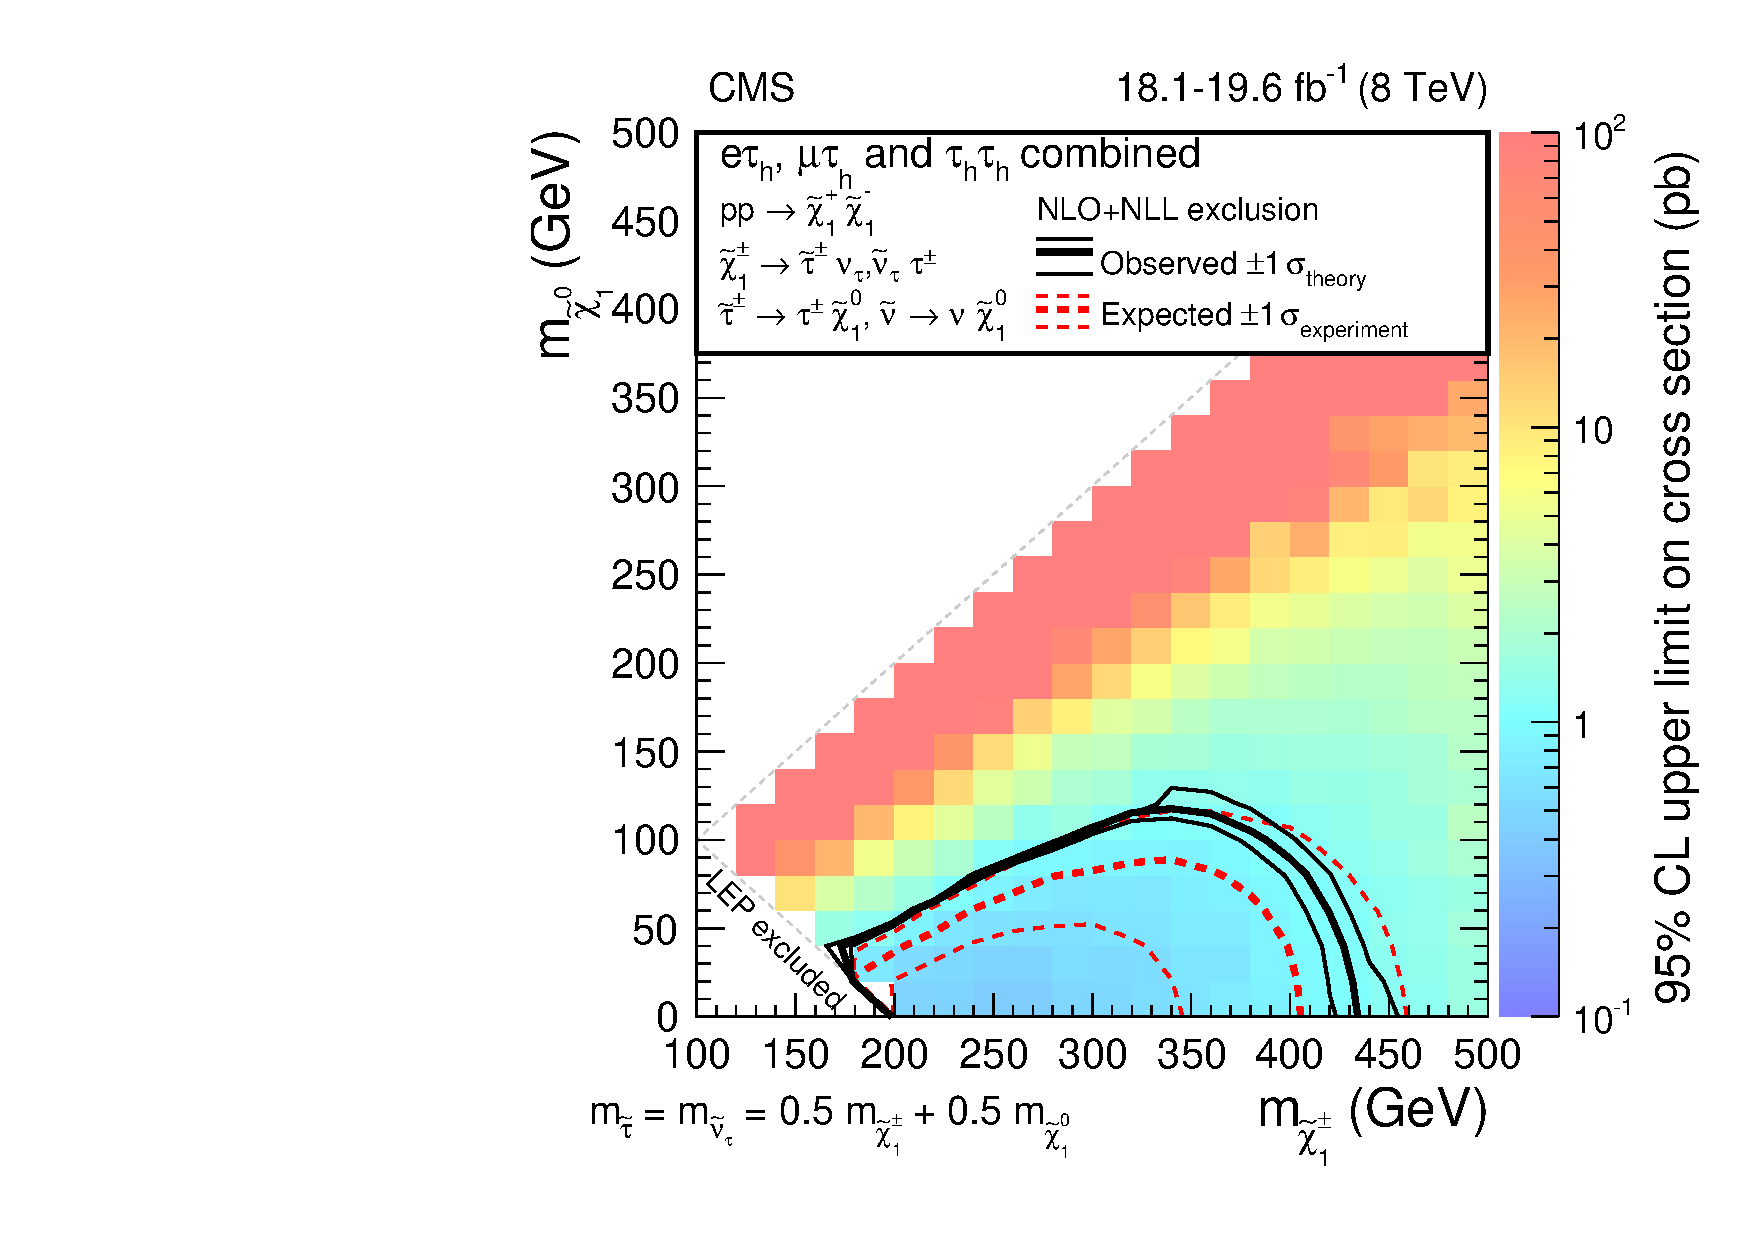
\includegraphics[width=0.7\textwidth,keepaspectratio=true]{StatisticsFig/Exclusion4Bins.pdf}
\caption{Expected and observed exclusion regions in terms of simplified models of
chargino pair production 
with the total data set of 2012. The bottom-left triangle was excluded by LEP \sTau searches.
The $\pm$1 standard deviation of the expected (observed) exclusions introduced by the experimental 
(theoretical) uncertainties are also shown.}
\label{fig:limit_final}
\end{figure}
\end{linenomath}
Combining all four signal regions,
the observed limits rule out \chione  masses up to  420\GeV  for a massless \PSGczDo.  
This can be compared to the ATLAS limit of 345\GeV for a massless \PSGczDo \cite{Aad:2014yka}.
It should be noted that the ATLAS results are based on the \tauTau channel alone. Figure 
\ref{fig:limit_tauTau} 
\begin{linenomath}
\begin{figure}[!htb]
\centering
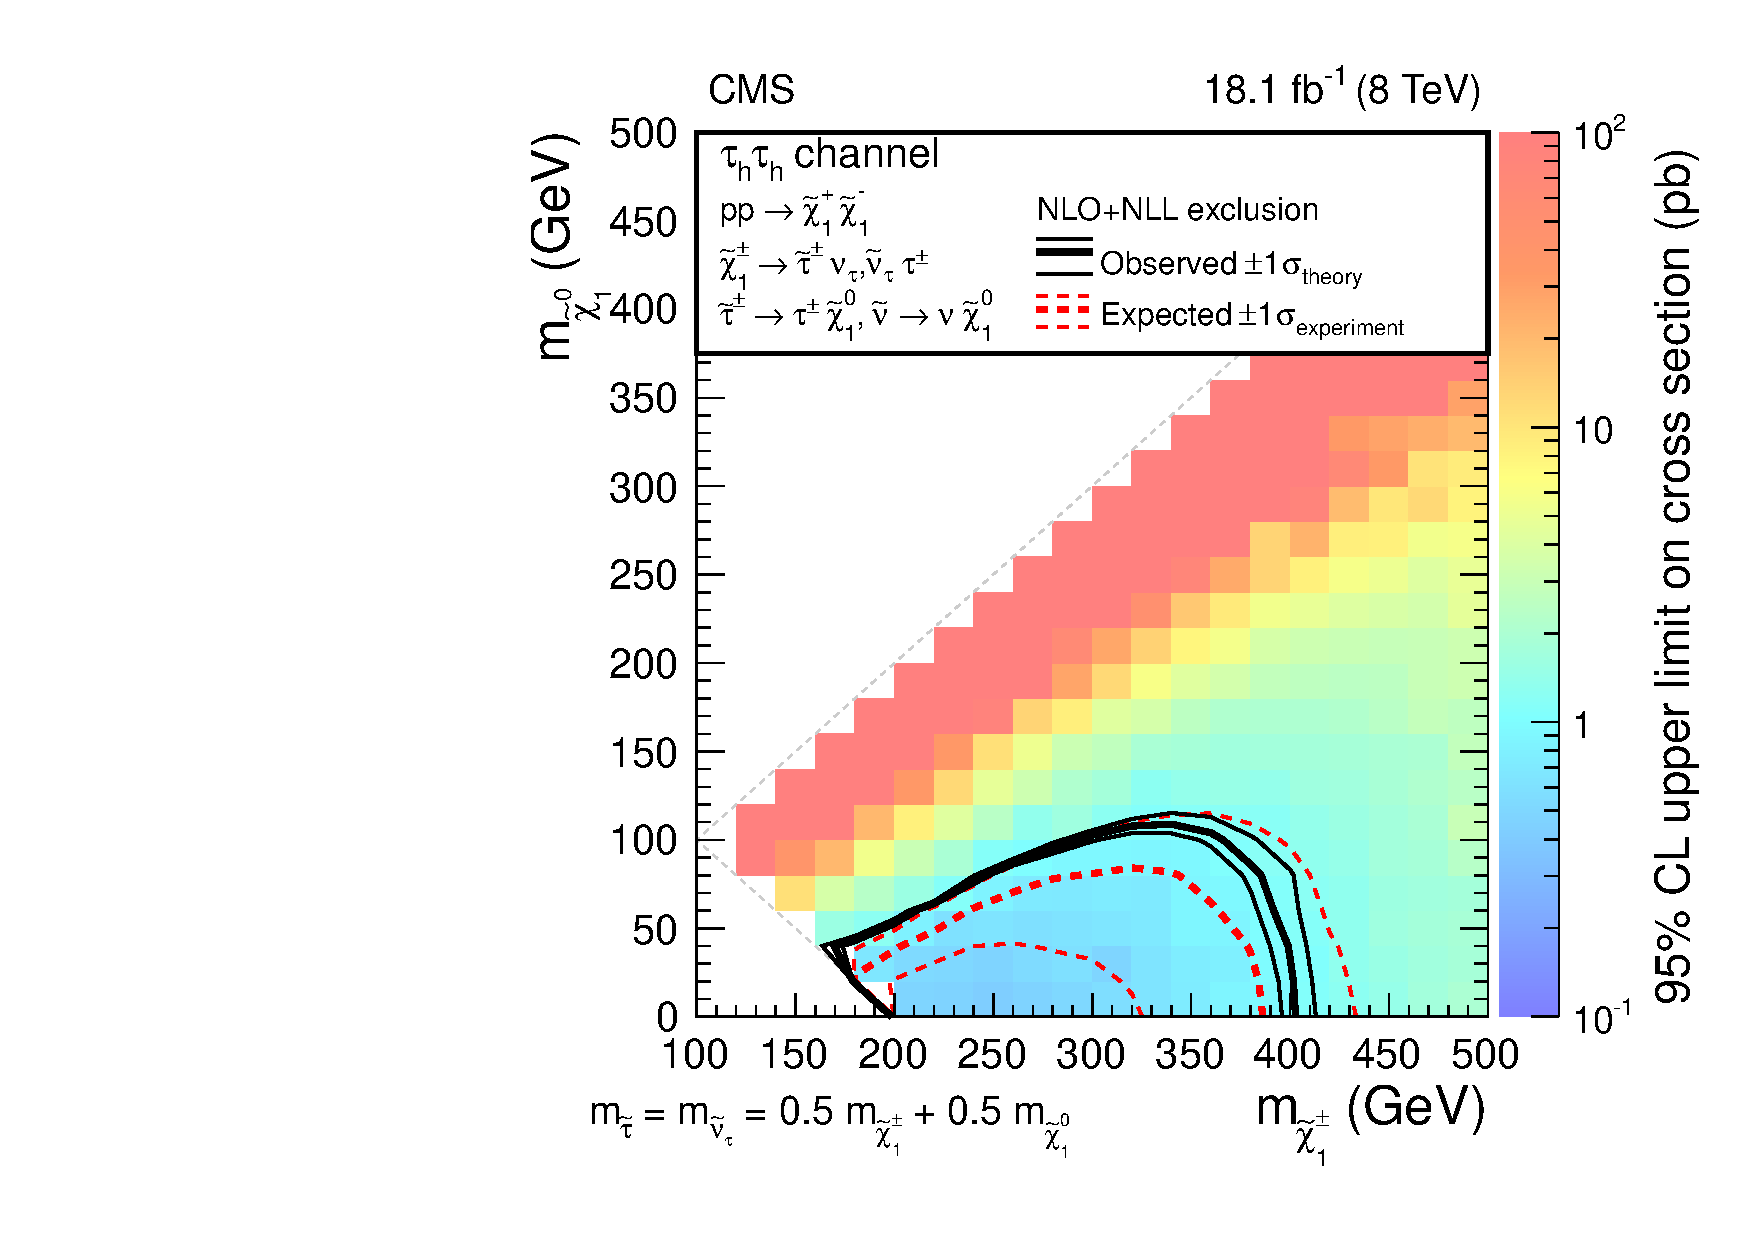
\includegraphics[width=0.7\textwidth,keepaspectratio=true]{StatisticsFig/ExclusionTauTau2Bin.pdf}
\caption{Expected and observed exclusion regions in terms of simplified models
in the \tauTau channel. The conventions are the same as Fig.~\ref{fig:limit_final}.}
\label{fig:limit_tauTau}
\end{figure}
\end{linenomath}
shows the results in the \tauTau channel, where the \chione masses are excluded up to 400\GeV for a massless \PSGczDo. 

The triangle in the bottom-left corner of Figs.~\ref{fig:limit_final} and 
\ref{fig:limit_tauTau} corresponds to  \sTau masses below 96\GeV, which has been excluded by the LEP experiments~\cite{lepsusy}.
%The \sTau searches in the LEP experiments \cite{lepsusy} have excluded \sTau masses below 95\GeV. In Figs.~\ref{fig:limit_final} and 
%\ref{fig:limit_tauTau}, this region corresponds to the triangle in bottom-left corner. 
%The diagonal line denotes the boundary for $m_{\chione} = m_{\tau} + m_{\neutralino}$, which is the kinematical boundary of the search.
The expected limits and the contours corresponding to $\pm$1 standard deviation from experimental uncertainties are shown as red lines. 
The observed limits are shown with a black solid line, 
while the $\pm$1 standard deviation based on the signal cross section uncertainties are shown with narrower black lines.
%The signal cross sections in NLO + NLL order in the strong coupling constant $\alpha_s$ are used to make the exclusion limits.
In the whole region, the observed limits are within one standard deviation of the expected limits.  


The results are also interpreted to set limits on $\sTau\sTau$ production, 
which corresponds to the right diagram in Fig.~\ref{fig:Productions}. 
In this simplified model, two \sTau particles are directly produced from the pp  collision and decay promptly to two $\tau$ leptons and two neutralinos. 
The effect of the two $\ell\Tau$ channels are found to be negligible and therefore are not considered.
To calculate the production cross section, \sTau is 
defined as a maximal admixture of the left-handed and right-handed \sTau gauge eigenstates \cite{Fuks:2013lya}. 
Since the cross section for direct production of sleptons is lower, no point is excluded and a $95\%$ CL upper limit is set on 
the cross section  as a function of the \sTau mass. 
Figure \ref{fig:limit_stau_stau} displays the ratio of the 
\begin{linenomath}
\begin{figure}[!htb]
\centering
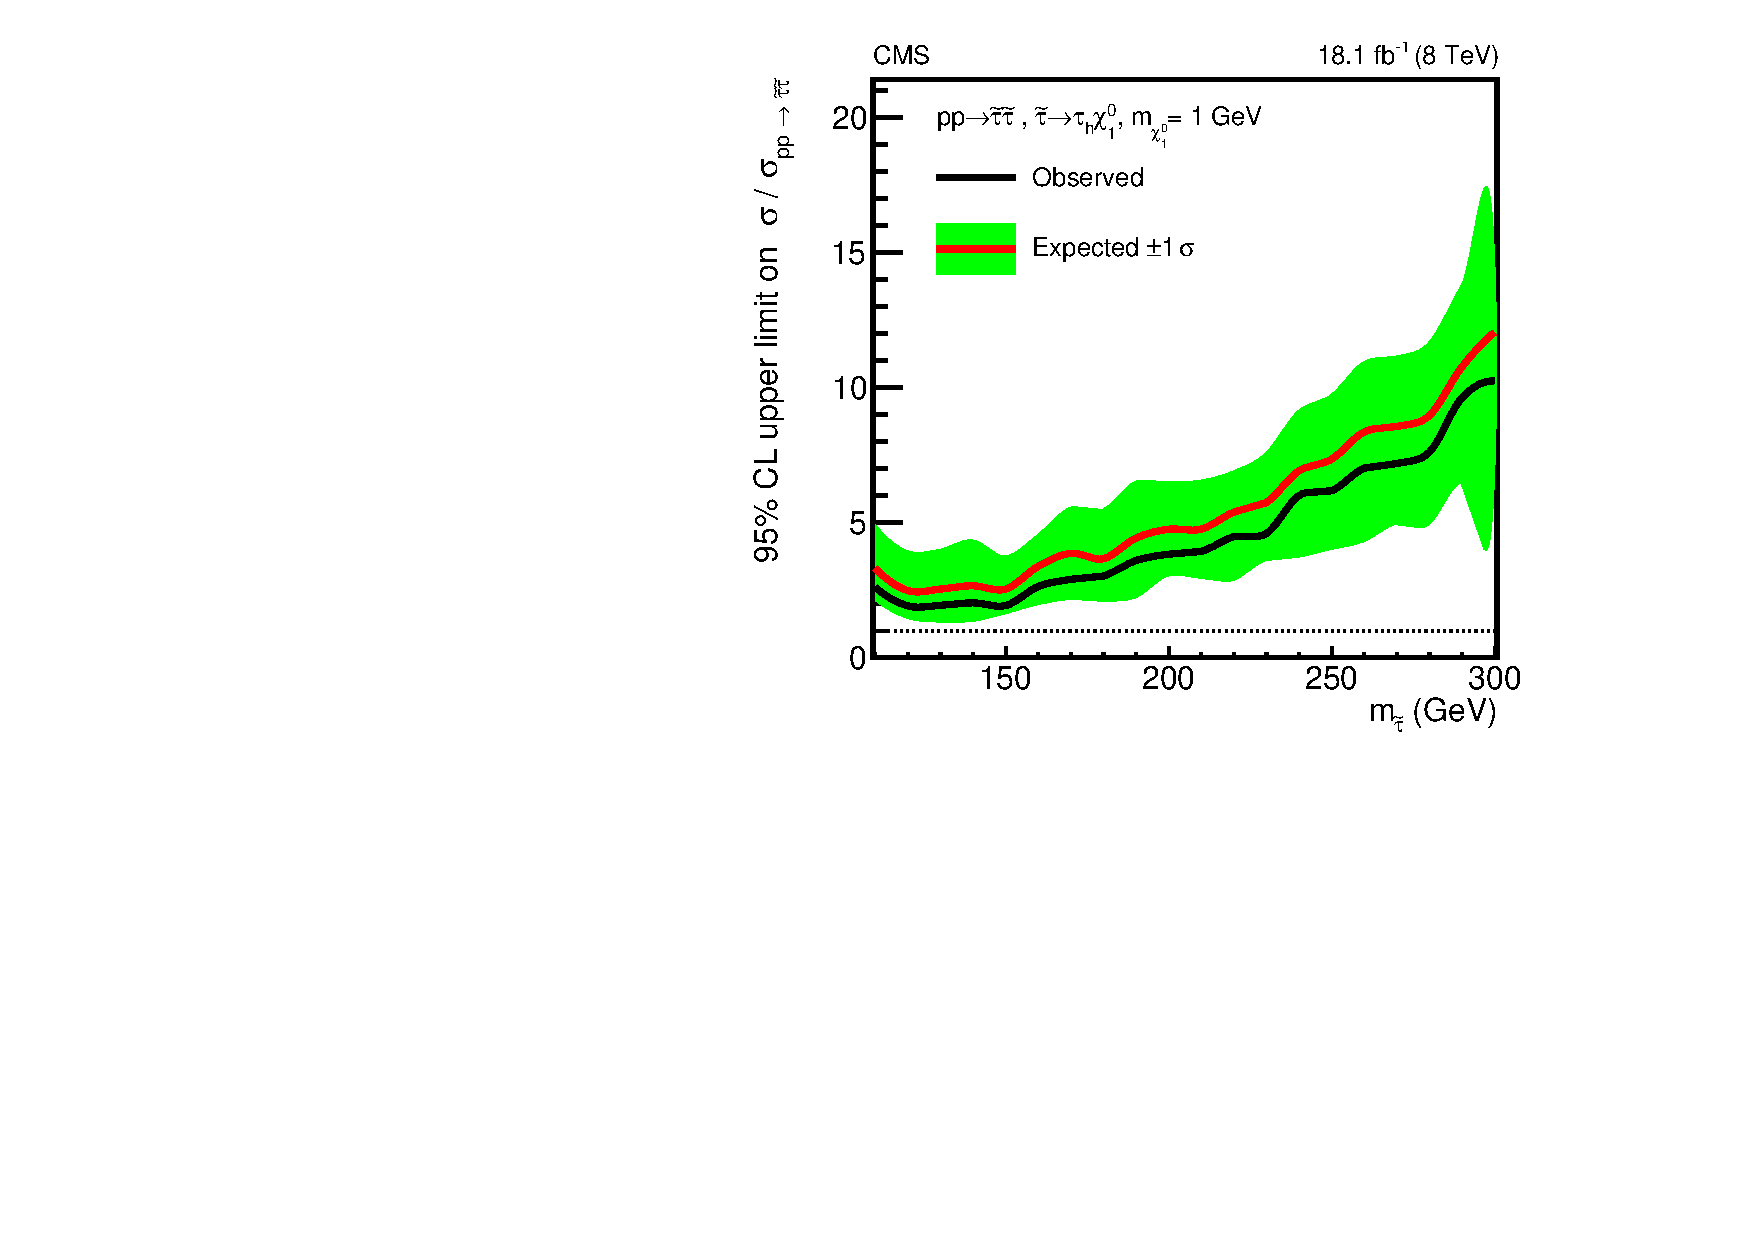
\includegraphics[width=1.0\textwidth,keepaspectratio=true]{StatisticsFig/ExclusionSTauSTauLsp1.pdf}
\caption{Upper limits at 95\% confidence level on $\sTau\sTau$ production cross section in the \tauTau channel. The mass of \PSGczDo is 1\GeV.}
\label{fig:limit_stau_stau}
\end{figure}
\end{linenomath}
obtained upper limit on the cross section and the cross section expected from SUSY (signal strength) versus the mass of the \sTau particle, with the \PSGczDo mass set to 1\GeV.
The observed limit is within one standard deviation of  the expected limit.
The best limit, which corresponds to the lowest signal strength, is obtained for $m_{\sTau}=150\GeV$. The observed (expected) upper limit on the cross section at this mass is 43 (56) fb which is almost two  times larger than the theoretical NLO prediction.



